\subsection{Reducing the Size of a Mesh}
\label{sec:removing}

The definition of discrete Gaussian curvature that we
derived by applying the Gauss-Bonnet theorem is used when 
a triangulated surface is generated by scanning an object.
In this context, a triangulated surface is called a mesh.

Meshes that are obtained by scanning real objects contain noise.
Most meshes that are generated by scanning require a complete
remeshing \cite{remeshing-2003}.
As a first step in remeshing, the curvature at each
vertex needs to be estimated \cite{mmsb-2003}.




Computing the curvature at each vertex in a mesh can allow one to reduce
the number of vertices in the mesh without sacrificing mesh quality.
This leads to simplification process that reduces storage space and improves the efficiency of
 algorithms run on the mesh.
If the curvature at a vertex is zero, then the vertex can be removed,
along with the faces and edges incident to the vertex, without changing 
the mesh.
 If the curvature is small, then few points
are sampled to be included in the re-mesh. If the curvature
is large, then many points are sampled. See \figref{planck-mesh}
for an illustration.

\begin{figure}[htb]
\centering
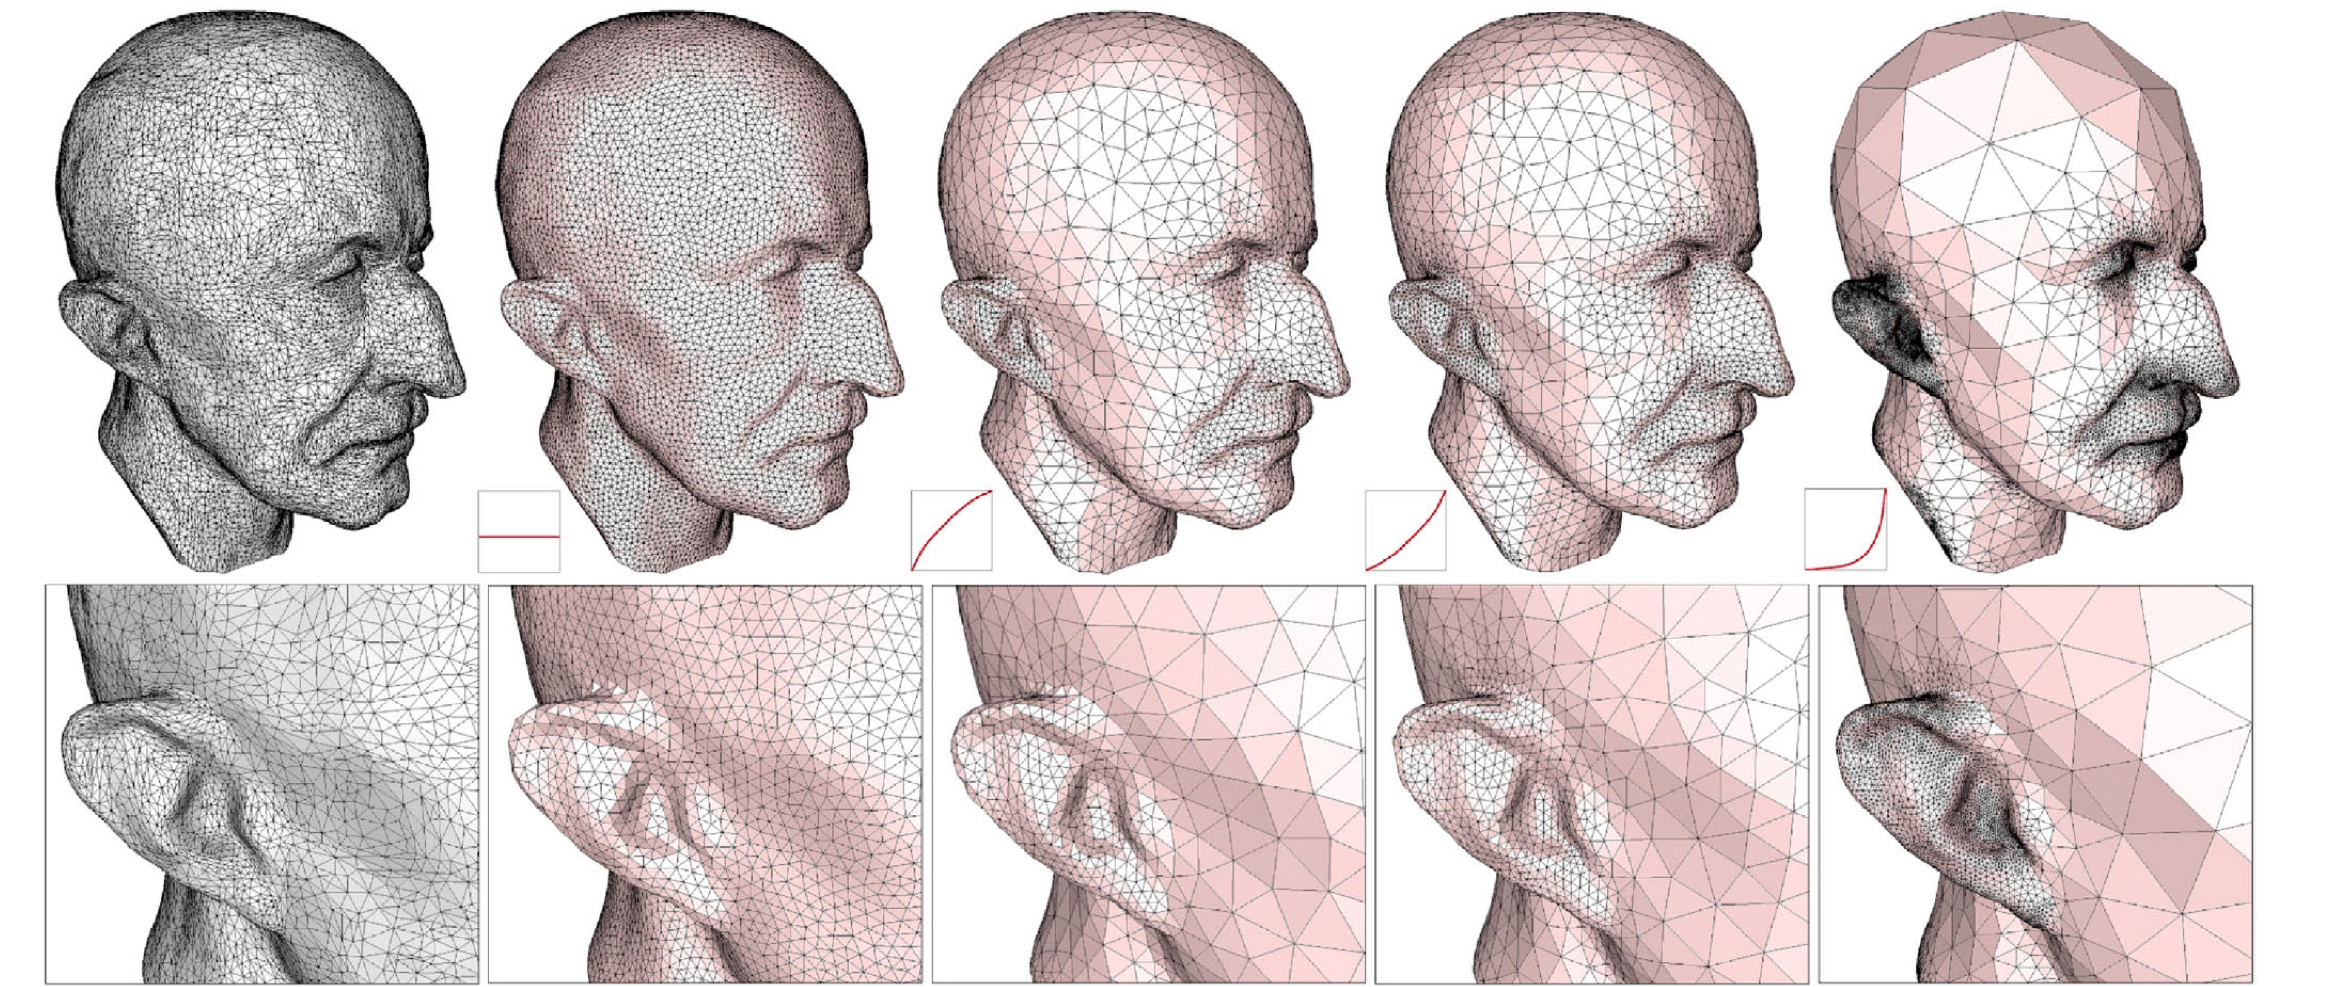
\includegraphics[width=.7\textwidth]{meshes/planck-mesh.jpeg}
\caption{A mesh of Max Plank. The original mesh is on the left. As we move
from left to right more importance is placed on vertices with large curvature.
Figure from \cite{alliez-2002}.}
\label{fig:planck-mesh}
\end{figure}


The experiments in \cite{mmsb-2003} found that the average
percent error did not exceed $1.3\%$ when using this operator.\todo{what does
this mean?}

